
\documentclass[letterpaper,hide notes,xcolor={table,svgnames},pdftex]{beamer}
\def\showexamples{t}


%\usepackage[svgnames]{xcolor}

%% Demo talk
%\documentclass[letterpaper,notes=show]{beamer}

\usecolortheme{crane}
\setbeamertemplate{navigation symbols}{}

\usetheme{MyPittsburgh}
%\usetheme{Frankfurt}

%\usepackage{tipa}

\usepackage{hyperref}
\usepackage{graphicx,xspace}
\usepackage[normalem]{ulem}

\newcommand\SF[1]{$\bigstar$\footnote{SF: #1}}



\newcounter{tmpnumSlide}
\newcounter{tmpnumNote}

% old question code
%\newcommand\question[1]{{$\bigstar$ \small \onlySlide{2}{#1}}}
% \newcommand\nquestion[1]{\ifdefined \presentationonly \textcircled{?} \fi \note{\par{\Large \textbf{?}} #1}}
% \newcommand\nanswer[1]{\note{\par{\Large \textbf{A}} #1}}


 \newcommand\mnote[1]{%
   \addtocounter{tmpnumSlide}{1}
   \ifdefined\showcues {~\tiny\fbox{\arabic{tmpnumSlide}}}\fi
   \note{\setlength{\parskip}{1ex}\addtocounter{tmpnumNote}{1}\textbf{\Large \arabic{tmpnumNote}:} {#1\par}}}

\newcommand\mmnote[1]{\note{\setlength{\parskip}{1ex}#1\par}}

%\newcommand\mnote[2][]{\ifdefined\handoutwithnotes {~\tiny\fbox{#1}}\fi
% \note{\setlength{\parskip}{1ex}\textbf{\Large #1:} #2\par}}

%\newcommand\mnote[2][]{{\tiny\fbox{#1}} \note{\setlength{\parskip}{1ex}\textbf{\Large #1:} #2\par}}

\newcommand\mquestion[2]{{~\color{red}\fbox{?}}\note{\setlength{\parskip}{1ex}\par{\Large \textbf{?}} #1} \note{\setlength{\parskip}{1ex}\par{\Large \textbf{A}} #2\par}\ifdefined \presentationonly \pause \fi}

\newcommand\blackboard[1]{%
\ifdefined   \showblackboard
  {#1}
  \else {\begin{center} \fbox{\colorbox{blue!30}{%
         \begin{minipage}{.95\linewidth}%
           \hspace{\stretch{1}} Some space intentionally left blank; done at the blackboard.%
         \end{minipage}}}\end{center}}%
         \fi%
}



%\newcommand\q{\tikz \node[thick,color=black,shape=circle]{?};}
%\newcommand\q{\ifdefined \presentationonly \textcircled{?} \fi}

\usepackage{listings}
\lstset{%
  keywordstyle=\bfseries,
  aboveskip=15pt,
  belowskip=15pt,
  captionpos=b,
  identifierstyle=\ttfamily,
  escapeinside={(*@}{@*)},
  stringstyle=\ttfamiliy,
  frame=lines,
  numbers=left, basicstyle=\scriptsize, numberstyle=\tiny, stepnumber=0, numbersep=2pt}

\usepackage{siunitx}
\newcommand\sius[1]{\num[group-separator = {,}]{#1}\si{\micro\second}}
\newcommand\sims[1]{\num[group-separator = {,}]{#1}\si{\milli\second}}
\newcommand\sins[1]{\num[group-separator = {,}]{#1}\si{\nano\second}}
\sisetup{group-separator = {,}, group-digits = true}

%% -------------------- tikz --------------------
\usepackage{tikz}
\usetikzlibrary{positioning}
\usetikzlibrary{arrows,backgrounds,automata,decorations.shapes,decorations.pathmorphing,decorations.markings,decorations.text}

\tikzstyle{place}=[circle,draw=blue!50,fill=blue!20,thick, inner sep=0pt,minimum size=6mm]
\tikzstyle{transition}=[rectangle,draw=black!50,fill=black!20,thick, inner sep=0pt,minimum size=4mm]

\tikzstyle{block}=[rectangle,draw=black, thick, inner sep=5pt]
\tikzstyle{bullet}=[circle,draw=black, fill=black, thin, inner sep=2pt]

\tikzstyle{pre}=[<-,shorten <=1pt,>=stealth',semithick]
\tikzstyle{post}=[->,shorten >=1pt,>=stealth',semithick]
\tikzstyle{bi}=[<->,shorten >=1pt,shorten <=1pt, >=stealth',semithick]

\tikzstyle{mut}=[-,>=stealth',semithick]

\tikzstyle{treereset}=[dashed,->, shorten >=1pt,>=stealth',thin]

\usepackage{ifmtarg}
\usepackage{xifthen}
\makeatletter
% new counter to now which frame it is within the sequence
\newcounter{multiframecounter}
% initialize buffer for previously used frame title
\gdef\lastframetitle{\textit{undefined}}
% new environment for a multi-frame
\newenvironment{multiframe}[1][]{%
\ifthenelse{\isempty{#1}}{%
% if no frame title was set via optional parameter,
% only increase sequence counter by 1
\addtocounter{multiframecounter}{1}%
}{%
% new frame title has been provided, thus
% reset sequence counter to 1 and buffer frame title for later use
\setcounter{multiframecounter}{1}%
\gdef\lastframetitle{#1}%
}%
% start conventional frame environment and
% automatically set frame title followed by sequence counter
\begin{frame}%
\frametitle{\lastframetitle~{\normalfont(\arabic{multiframecounter})}}%
}{%
\end{frame}%
}
\makeatother

\makeatletter
\newdimen\tu@tmpa%
\newdimen\ydiffl%
\newdimen\xdiffl%
\newcommand\ydiff[2]{%
    \coordinate (tmpnamea) at (#1);%
    \coordinate (tmpnameb) at (#2);%
    \pgfextracty{\tu@tmpa}{\pgfpointanchor{tmpnamea}{center}}%
    \pgfextracty{\ydiffl}{\pgfpointanchor{tmpnameb}{center}}%
    \advance\ydiffl by -\tu@tmpa%
}
\newcommand\xdiff[2]{%
    \coordinate (tmpnamea) at (#1);%
    \coordinate (tmpnameb) at (#2);%
    \pgfextractx{\tu@tmpa}{\pgfpointanchor{tmpnamea}{center}}%
    \pgfextractx{\xdiffl}{\pgfpointanchor{tmpnameb}{center}}%
    \advance\xdiffl by -\tu@tmpa%
}
\makeatother
\newcommand{\copyrightbox}[3][r]{%
\begin{tikzpicture}%
\node[inner sep=0pt,minimum size=2em](ciimage){#2};
\usefont{OT1}{phv}{n}{n}\fontsize{4}{4}\selectfont
\ydiff{ciimage.south}{ciimage.north}
\xdiff{ciimage.west}{ciimage.east}
\ifthenelse{\equal{#1}{r}}{%
\node[inner sep=0pt,right=1ex of ciimage.south east,anchor=north west,rotate=90]%
{\raggedleft\color{black!50}\parbox{\the\ydiffl}{\raggedright{}#3}};%
}{%
\ifthenelse{\equal{#1}{l}}{%
\node[inner sep=0pt,right=1ex of ciimage.south west,anchor=south west,rotate=90]%
{\raggedleft\color{black!50}\parbox{\the\ydiffl}{\raggedright{}#3}};%
}{%
\node[inner sep=0pt,below=1ex of ciimage.south west,anchor=north west]%
{\raggedleft\color{black!50}\parbox{\the\xdiffl}{\raggedright{}#3}};%
}
}
\end{tikzpicture}
}


%% --------------------

%\usepackage[excludeor]{everyhook}
%\PushPreHook{par}{\setbox0=\lastbox\llap{MUH}}\box0}

%\vspace*{\stretch{1}

%\setbox0=\lastbox \llap{\textbullet\enskip}\box0}

\setlength{\parskip}{\fill}

\newcommand\noskips{\setlength{\parskip}{1ex}}
\newcommand\doskips{\setlength{\parskip}{\fill}}

\newcommand\xx{\par\vspace*{\stretch{1}}\par}
\newcommand\xxs{\par\vspace*{2ex}\par}
\newcommand\tuple[1]{\langle #1 \rangle}
\newcommand\code[1]{{\sf \footnotesize #1}}
\newcommand\ex[1]{\uline{Example:} \ifdefined \presentationonly \pause \fi
  \ifdefined\showexamples#1\xspace\else{\uline{\hspace*{2cm}}}\fi}

\newcommand\ceil[1]{\lceil #1 \rceil}


\AtBeginSection[]
{
   \begin{frame}
       \frametitle{Outline}
       \tableofcontents[currentsection]
   \end{frame}
}



\pgfdeclarelayer{edgelayer}
\pgfdeclarelayer{nodelayer}
\pgfsetlayers{edgelayer,nodelayer,main}

\tikzstyle{none}=[inner sep=0pt]
\tikzstyle{rn}=[circle,fill=Red,draw=Black,line width=0.8 pt]
\tikzstyle{gn}=[circle,fill=Lime,draw=Black,line width=0.8 pt]
\tikzstyle{yn}=[circle,fill=Yellow,draw=Black,line width=0.8 pt]
\tikzstyle{empty}=[circle,fill=White,draw=Black]
\tikzstyle{bw} = [rectangle, draw, fill=blue!20, 
    text width=4em, text centered, rounded corners, minimum height=2em]
    
    \newcommand{\CcNote}[1]{% longname
	This work is licensed under the \textit{Creative Commons #1 3.0 License}.%
}
\newcommand{\CcImageBy}[1]{%
	\includegraphics[scale=#1]{creative_commons/cc_by_30.pdf}%
}
\newcommand{\CcImageSa}[1]{%
	\includegraphics[scale=#1]{creative_commons/cc_sa_30.pdf}%
}
\newcommand{\CcImageNc}[1]{%
	\includegraphics[scale=#1]{creative_commons/cc_nc_30.pdf}%
}
\newcommand{\CcGroupBySa}[2]{% zoom, gap
	\CcImageBy{#1}\hspace*{#2}\CcImageNc{#1}\hspace*{#2}\CcImageSa{#1}%
}
\newcommand{\CcLongnameByNcSa}{Attribution-NonCommercial-ShareAlike}

\newenvironment{changemargin}[1]{% 
  \begin{list}{}{% 
    \setlength{\topsep}{0pt}% 
    \setlength{\leftmargin}{#1}% 
    \setlength{\rightmargin}{1em}
    \setlength{\listparindent}{\parindent}% 
    \setlength{\itemindent}{\parindent}% 
    \setlength{\parsep}{\parskip}% 
  }% 
  \item[]}{\end{list}} 





\title{Lecture 4 --- Java III}

\author{Jeff Zarnett \\ \small \texttt{jzarnett@uwaterloo.ca}}
\institute{Department of Electrical and Computer Engineering \\
  University of Waterloo}
\date{\today}


\begin{document}


\begin{frame}
  \titlepage
\end{frame}

\part{Exceptions, Annotations, \& I/O}
\frame{\partpage}

\begin{frame}
\frametitle{Exceptions}
\begin{changemargin}{1cm}

\texttt{Exception}s are used to signal an error (something unusual) during the execution of a program.

This disrupts the normal flow of the program's instructions.

An \texttt{Exception} is ``thrown'' when it is generated.

The keyword is \texttt{throw}.

\end{changemargin}
\end{frame}

\begin{frame}
\frametitle{Exceptions}
\begin{changemargin}{1cm}

Exceptions are generated automatically or explicitly in a program.

Write: \texttt{throw new RuntimeException(...)}

The JRE may also generate an exception:

Call \texttt{toString()} on an object that is null. JRE throws a \texttt{NullPointerException}.


\end{changemargin}
\end{frame}

\begin{frame}
\frametitle{Handling the Exception}
\begin{changemargin}{1cm}

If there is no code to ``handle'' this exception, then it goes up one level to the caller of that method until it gets to \texttt{main}. 

If \texttt{main} cannot deal with it either, then execution of the program will be stopped.

An error message will be printed on the screen. 

How to handle the exception? With an exception handler. 

\end{changemargin}
\end{frame}

\begin{frame}[fragile]
\frametitle{Catching Exceptions}
\begin{changemargin}{1cm}

Given that an \texttt{Exception} is \texttt{throw}n, it should come as no surprise that the keyword to handle it is \texttt{catch}. 

We demarcate code that a \texttt{catch} block is supposed to apply to in a \texttt{try} block. 

\begin{verbatim}
try {
  // Some statements   
} catch (Exception e) {
  // Handle the Exception
}
\end{verbatim}

\end{changemargin}
\end{frame}


\begin{frame}[fragile]
\frametitle{Try-Catch Block}
\begin{changemargin}{1cm}

Let's look at an example:

\begin{verbatim}
public void handleException() {
  Object example = null;
  try {
    System.out.println(example.toString());
  } catch (NullPointerException npe) {
    // Handle the NPE
  }
}
\end{verbatim}

\end{changemargin}
\end{frame}

\begin{frame}
\frametitle{Dealing with the Exception}
\begin{changemargin}{1cm}

Handling an exception depends on the specific program. 

Sometimes you might just display an error message.

In some cases you don't even want to handle the error.

Maybe the output contains information to find the problem. 

\end{changemargin}
\end{frame}

\begin{frame}[fragile]
\frametitle{Multiple Catch Blocks}
\begin{changemargin}{1cm}

\begin{verbatim}
try {
  // Some statements   
} catch (NullPointerException e) {
  // Handle the Exception
} catch (IOException e2) {
  // Do Something Else
} catch (FileNotFoundException | SQLException e3) {
  // Some other things
}
\end{verbatim}

\end{changemargin}
\end{frame}

\begin{frame}
\frametitle{The Finally Block}
\begin{changemargin}{1cm}

Optionally, after the catch block: the \texttt{finally} block. 

The finally block always executes when the try block exits, whether it went to the catch block or not. 

Use: avoid having cleanup code accidentally bypassed by a \texttt{return}, \texttt{continue}, or \texttt{break}.

\end{changemargin}
\end{frame}


\begin{frame}[fragile]
\frametitle{Finally Block Format}
\begin{changemargin}{1cm}
\begin{verbatim}
try {
  // Some statements   
} catch (Exception e) {
  // Handle the Exception
} finally {
  // Cleanup
}
\end{verbatim}
\end{changemargin}
\end{frame}

\begin{frame}[fragile]
\frametitle{Finally Blocks}
\begin{changemargin}{1cm}
What is the return value of this function?

\begin{verbatim}
public boolean tryFinally() {
  try {
    return false;
  } finally {
    return true;
  }
}
\end{verbatim}
\end{changemargin}
\end{frame}

\begin{frame}[fragile]
\frametitle{Exceptions: Putting it Together}
\begin{changemargin}{1cm}
{\scriptsize
\begin{verbatim}
public void writeList() {
    PrintWriter out = null;

    try {
        System.out.println("Entering" + " try statement");

        out = new PrintWriter(new FileWriter("OutFile.txt"));
        for (int i = 0; i < SIZE; i++)
            out.println("Value at: " + i + " = " + vector.elementAt(i));
                  
    } catch (ArrayIndexOutOfBoundsException e) {
        System.err.println("Caught ArrayIndexOutOfBoundsException: "
                           +  e.getMessage());
                                 
    } catch (IOException e) {
        System.err.println("Caught IOException: " +  e.getMessage());
                                 
    } finally {
        if (out != null) {
            System.out.println("Closing PrintWriter");
            out.close();
        } 
        else {
            System.out.println("PrintWriter not open");
        }
    }
}
\end{verbatim}
}

\end{changemargin}
\end{frame}

\begin{frame}
\frametitle{Exception Example}
\begin{changemargin}{1cm}

\textbf{Scenario 1}: Exception Occurs

The \texttt{FileWriter} throws an \texttt{IOException}, because the file OutFile.txt is missing or inaccessible. 

Execution of the lines in the try block stops. 

The JRE then starts looking for a handler. 

It finds the catch block that specifies the IOException. 

The catch block is executed. 

Then the finally block executes.

\end{changemargin}
\end{frame}


\begin{frame}
\frametitle{Exception Example}
\begin{changemargin}{1cm}

\textbf{Scenario 2}: Everything Goes Well 

Suppose no exception occurs. 

Then the lines of the try block are all executed.

Then the finally block executes.

\end{changemargin}
\end{frame}

\begin{frame}
\frametitle{Exception Handling}
\begin{changemargin}{1cm}


Sometimes we don't want to handle an exception ourselves; sometimes we want to ``pass the buck''. 

To do that, declare that your method \texttt{throws} an exception:

\texttt{public void writeList() throws IOException}.


Then handling the \texttt{IOException} is the responsibility of whatever method calls \texttt{writeList()}.

\end{changemargin}
\end{frame}

\begin{frame}
\frametitle{Creating Exceptions}
\begin{changemargin}{1cm}

Want to create an exception in your code? 

Use the \texttt{throw} keyword. 

\texttt{throw new RunTimeException()}

Throw whatever type of exception is appropriate.

\end{changemargin}
\end{frame}

\begin{frame}
\frametitle{Final Thoughts on Exceptions}
\begin{changemargin}{1cm}

As a final note, exceptions are supposed to be exceptional.

Don't use them as part of the expected flow of your program. 

Use them to handle error conditions \& unexpected situations.

\end{changemargin}
\end{frame}

\begin{frame}
\frametitle{Eclipse: Stack Traces}
\begin{changemargin}{1cm}

Eclipse demo time: stack traces.

What happens when an exception occurs, what a stack trace looks like, and how to find the error using one.

\end{changemargin}
\end{frame}



\begin{frame}
\frametitle{Annotations}
\begin{changemargin}{1cm}

We've already seen some annotations. 

When we override a method from a superclass, we put the annotation \texttt{@Override} above it. 

Annotations start with the \texttt{@}-symbol and can be attached to methods, classes, and variables. 

\end{changemargin}
\end{frame}

\begin{frame}
\frametitle{Annotations}
\begin{changemargin}{1cm}

Meta-data; have no direct effect on the operation of the code.

They can be used for:

\begin{itemize}
	\item Information for the Compiler
	\item Compile-Time Processing
	\item Runtime Processing
\end{itemize}


\end{changemargin}
\end{frame}


\begin{frame}[fragile]
\frametitle{Basic Annotation}
\begin{changemargin}{1cm}

\begin{verbatim}
@Override
public void doSomething() { ... }
\end{verbatim}

Multiple annotations can appear on an element, and annotations can have properties, such as:

\begin{verbatim}
@Author(name = ''Alice'')
@EBook
public void doSomething() { ... }
\end{verbatim}

\end{changemargin}
\end{frame}

\begin{frame}
\frametitle{Annotations}
\begin{changemargin}{1cm}

You can write your own annotations, but the only one you are likely to need is the \texttt{@Override} annotation. 

\end{changemargin}
\end{frame}


\begin{frame}
\frametitle{Java Input/Output}
\begin{changemargin}{1cm}

In Java, Input/Output (or I/O) is modelled as a \textit{Stream}.

A Stream is a sequence of data. 

A stream can be used to read data (input stream) or write data (output stream). 


\end{changemargin}
\end{frame}

\begin{frame}
\frametitle{InputStream}
\begin{changemargin}{1cm}

\begin{center}
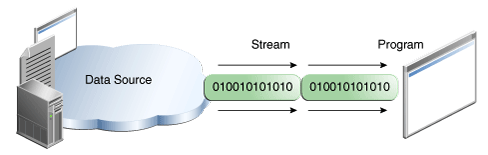
\includegraphics[width=0.85\textwidth]{images/inputstream.png}
\end{center}

\end{changemargin}
\end{frame}

\begin{frame}
\frametitle{OutputStream}
\begin{changemargin}{1cm}

\begin{center}
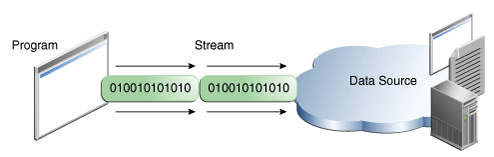
\includegraphics[width=0.85\textwidth]{images/outputstream.png}
\end{center}

\end{changemargin}
\end{frame}

\begin{frame}
\frametitle{Streams}
\begin{changemargin}{1cm}

The classes used to do I/O are descendants of the superclasses \texttt{InputStream} or \texttt{OutputStream}. 

For example, to read from a file, use a \texttt{FileInputStream}. 

\end{changemargin}
\end{frame}

\begin{frame}[fragile]
\frametitle{Reading a File and Writing it Again}
\begin{changemargin}{1cm}
{\scriptsize
\begin{verbatim}
public class CopyFile {
    public static void main(String[] args) throws IOException {

        FileInputStream in = null;
        FileOutputStream out = null;

        try {
            in = new FileInputStream("input.txt");
            out = new FileOutputStream("output.txt");
            int c;

            while ((c = in.read()) != -1) {
                out.write(c);
            }
        } finally {
            if (in != null) {
                in.close();
            }
            if (out != null) {
                out.close();
            }
        }
    }
}
\end{verbatim}
}
\end{changemargin}
\end{frame}

\begin{frame}
\frametitle{Comments on File Copier}
\begin{changemargin}{1cm}

Note that the file streams are closed inside the \texttt{finally} block.

They will be closed even if something goes wrong. 

This works, but it's really, really inefficient. Why? 

We are reading from the disk one character (one byte) at a time and that's really slow. 

What we'd often like to do is read a whole line at once. 

\end{changemargin}
\end{frame}

\begin{frame}[fragile]
\frametitle{Reading a Line at a Time}
\begin{changemargin}{1cm}
{\scriptsize
\begin{verbatim}
public class CopyFile {
    public static void main(String[] args) throws IOException {

        BufferedReader inputStream = null;
        PrintWriter outputStream = null;

        try {
            inputStream = new BufferedReader(new FileReader("input.txt"));
            outputStream = new PrintWriter(new FileWriter("output.txt"));

            String l;
            while ((l = inputStream.readLine()) != null) {
                outputStream.println(l);
            }
        } finally {
            if (inputStream != null) {
                inputStream.close();
            }
            if (outputStream != null) {
                outputStream.close();
            }
        }
    }
}
\end{verbatim}
}

\end{changemargin}
\end{frame}

\begin{frame}
\frametitle{Buffered Reader}
\begin{changemargin}{1cm}

We also use a \texttt{BufferedReader} to get buffered I/O. 

When we read one byte at a time, each read or write request for an individual byte results in going to the disk or network.

When we work with buffered I/O, we read a buffer (some array of data) and store it. 

Then when we try to read a byte we check if it's in the array we already have stored. 

If so, se that value instead of going to the disk. 

When we reach the end of the buffer, fill up the buffer again.

\end{changemargin}
\end{frame}


\begin{frame}
\frametitle{Buffered Writer}
\begin{changemargin}{1cm}

Buffered output streams mean that output is kept in a buffer and only written to disk when the buffer is full. 

A crash might terminate execution before the buffer is written to disk and some of the expected output will not appear. 

To force the buffer to output its data, you can call \texttt{flush()}.

Closing the stream also has the effect of flushing the buffer.

\end{changemargin}
\end{frame}


\begin{frame}
\frametitle{Other Kinds of Streams}
\begin{changemargin}{1cm}

Java also has data streams and object streams, which are used for reading/writing/storing/loading more complex things. 

They are beyond the scope of this course.
\end{changemargin}
\end{frame}










\part{On Problem Solving}
\frame{\partpage}

\begin{frame}
\frametitle{The Key to Programming}
\begin{changemargin}{1cm}
The key to programming is simple.

\begin{enumerate}
\item Determine where we are (point A).
\item Determine where we're trying to go (point B).
\item Find a series of steps to get us from A to B.
\end{enumerate}

\end{changemargin}
\end{frame}

\begin{frame}
\frametitle{Math Problem Example}
\begin{changemargin}{1cm}

Suppose you haven't memorized the answer to $12 \times 13$. 

Other than whipping out the calculator, what can you do? 

Break it down into a series of problems you know how to solve.

$(12 x 10) + (12 x 3)$

We now have three problems, but they're small and easy.

\end{changemargin}
\end{frame}

\begin{frame}
\frametitle{Decomposition}
\begin{changemargin}{1cm}

Note: we have to know the rules of math to understand how the problem can be decomposed. 

In programming, the step you come up with might be a little bit too complicated for a computer or person to execute.

So you break the items of step 3 down by repeating this process.

Keep breaking it down until the steps are small enough for the computer to execute.

\end{changemargin}
\end{frame}

\begin{frame}
\frametitle{Decomposition: Step Size}
\begin{changemargin}{1cm}

How small those steps are is a matter of what language and tools you are using. 

Imagine a Fourier Transform of a signal (fancy math). 

If you're using an advanced language you might just write \texttt{FourierTransform(signal)}.

Or you might have to write the transform at a low level.

\end{changemargin}
\end{frame}

\begin{frame}
\frametitle{Key Lesson}
\begin{changemargin}{1cm}

Decomposing the problem is the key.

Learning the syntax of the language is another matter...

\end{changemargin}
\end{frame}


\end{document}

